\documentclass[11pt,a4paper]{article} 

%------------------------------------------------------------------------------
%	REQUIRED PACKAGES AND  CONFIGURATIONS
%------------------------------------------------------------------------------

\usepackage{titling}
\usepackage{tocloft}
\usepackage{booktabs}
\usepackage{multirow}

% PACKAGES FOR TITLES
\usepackage{titlesec}
\usepackage{color}

% PACKAGES FOR LANGUAGE AND FONT
\usepackage[utf8]{inputenc}
\usepackage[italian]{babel}
\usepackage[T1]{fontenc} % Font encoding
%\usepackage{FiraMono}
\usepackage{inconsolata}

% PACKAGES FOR IMAGES
\usepackage{graphicx}
\graphicspath{{Images/}}
\usepackage{eso-pic} % For the background picture on the title page
\usepackage{subfig} % Numbered and caption subfigures using \subfloat
\usepackage{caption} % Coloured captions
\usepackage{transparent}

% STANDARD MATH PACKAGES
\usepackage{amsmath}
\usepackage{amsthm}
\usepackage{bm}
\usepackage[overload]{empheq}  % For braced-style systems of equations

% PACKAGES FOR TABLES
\usepackage{tabularx}
\usepackage{longtable} % tables that can span several pages
\usepackage{colortbl}

% PACKAGES FOR ALGORITHMS (PSEUDO-CODE)
\usepackage{algorithm}
\usepackage{algorithmic}

% PACKAGES FOR REFERENCES & BIBLIOGRAPHY
\usepackage[colorlinks=true,linkcolor=black,anchorcolor=black,citecolor=black,filecolor=black,menucolor=black,runcolor=black,urlcolor=black]{hyperref} % Adds clickable links at references
\usepackage{cleveref}
\usepackage[square, numbers, sort&compress]{natbib} % Square brackets, citing references with numbers, citations sorted by appearance in the text and compressed
\bibliographystyle{plain} % You may use a different style adapted to your field

% PACKAGES FOR THE APPENDIX
\usepackage{appendix}

% PACKAGES FOR ITEMIZE & ENUMERATES 
\usepackage{enumitem}

% OTHER PACKAGES
\usepackage{amsthm,thmtools,xcolor} % Coloured "Theorem"
\usepackage{comment} % Comment part of code
\usepackage{fancyhdr} % Fancy headers and footers
\usepackage{lipsum} % Insert dummy text
\usepackage{tcolorbox} % Create coloured boxes (e.g. the one for the key-words)

%-------------------------------------------------------------------------
%	NEW COMMANDS DEFINED
%-------------------------------------------------------------------------
% EXAMPLES OF NEW COMMANDS -> here you see how to define new commands
\newcommand{\bea}{\begin{eqnarray}} % Shortcut for equation arrays
\newcommand{\eea}{\end{eqnarray}}
\newcommand{\e}[1]{\times 10^{#1}}  % Powers of 10 notation
\newcommand{\mathbbm}[1]{\text{\usefont{U}{bbm}{m}{n}#1}} % From mathbbm.sty
\newcommand{\pdev}[2]{\frac{\partial#1}{\partial#2}}
%\newcommand{\m}[1]{{\fontfamily{fvm}\selectfont #1}}
\newcommand{\m}[1]{{\fontfamily{zi4}\selectfont #1}}

% NB: you can also override some existing commands with the keyword \renewcommand

%----------------------------------------------------------------------------
%	ADD YOUR PACKAGES (be careful of package interaction)
%----------------------------------------------------------------------------


%----------------------------------------------------------------------------
%	ADD YOUR DEFINITIONS AND COMMANDS (be careful of existing commands)
%----------------------------------------------------------------------------


% Do not change Configuration_files/config.tex file unless you really know what you are doing. 
% This file ends the configuration procedures (e.g. customizing commands, definition of new commands)
% Configuration package
\usepackage[bottom=2.0cm,top=2.0cm,left=2.0cm,right=2.0cm]{geometry}
\raggedbottom

% Create color bluePoli (-> manuale grafica coordinata:  https://www.polimi.it/fileadmin/user_upload/il_Politecnico/grafica-coordinata/2015_05_11_46xy_manuale_grafica_coordinata.pdf)
\definecolor{bluePoli}{cmyk}{0.4,0.1,0,0.4}

% Custom theorem environments
\declaretheoremstyle[
	headfont=\color{bluePoli}\normalfont\bfseries,
	bodyfont=\color{black}\normalfont\itshape,
]{colored}

\captionsetup[figure]{labelfont={color=bluePoli}} % Set colour of the captions
\captionsetup[table]{labelfont={color=bluePoli}} % Set colour of the captions
% \captionsetup[algorithm]{labelfont={color=bluePoli}} % Set colour of the captions

\theoremstyle{colored}
\newtheorem{theorem}{Theorem}[section]
\newtheorem{proposition}{Proposition}[section]

% Enhances the features of the standard "table" and "tabular" environments.
\newcommand\T{\rule{0pt}{2.6ex}}
\newcommand\B{\rule[-1.2ex]{0pt}{0pt}}

% Algorithm description
\newcounter{algsubstate}
\renewcommand{\thealgsubstate}{\alph{algsubstate}}
\newenvironment{algsubstates}{
	\setcounter{algsubstate}{0}%
	\renewcommand{\STATE}{%
		\stepcounter{algsubstate}%
		\Statex {\small\thealgsubstate:}\space}
}{}

% Custom theorem environment
\newcolumntype{L}[1]{>{\raggedright\let\newline\\\arraybackslash\hspace{0pt}}m{#1}}
\newcolumntype{C}[1]{>{\centering\let\newline\\\arraybackslash\hspace{0pt}}m{#1}}
\newcolumntype{R}[1]{>{\raggedleft\let\newline\\\arraybackslash\hspace{0pt}}m{#1}}

% Custom itemize environment
\setlist[itemize,1]{label=$\bullet$}
\setlist[itemize,2]{label=$\circ$}
\setlist[itemize,3]{label=$-$}
\setlist{nosep}

% Create command for background pic
\newcommand\BackgroundPic{% Adding background picture
	\put(237,365){
		\parbox[b][\paperheight]{\paperwidth}{%
			\vfill
			\centering
			\transparent{0.4}
			
\includegraphics[width=0.44\paperwidth]{raggiera_polimi.eps}%
			\vfill}
	}
}

% Set indentation
\setlength\parindent{0pt}

% Custom title commands
\titleformat{\section}
{\color{bluePoli}\normalfont\Large\bfseries}
{\color{bluePoli}\thesection.}{1em}{}
\titlespacing*{\section}
{0pt}{3.3ex}{3.3ex}

\titleformat{\subsection}
{\color{bluePoli}\normalfont\large\bfseries}
{\color{bluePoli}\thesubsection.}{1em}{}
\titlespacing*{\subsection}
{0pt}{3.3ex}{3.3ex}

\titleformat{\subsubsection}
{\color{bluePoli}\normalfont\large\bfseries}
{\color{bluePoli}\thesubsubsection.}{1em}{}
\titlespacing*{\subsection}
{0pt}{3.3ex}{3.3ex}

% Custom headers and footers
\pagestyle{fancy}
\fancyhf{}

\fancyfoot{}
\fancyfoot[C]{\thepage} % page
\renewcommand{\headrulewidth}{0mm} % headrule width
\renewcommand{\footrulewidth}{0mm} % footrule width

\makeatletter
\patchcmd{\headrule}{\hrule}{\color{black}\hrule}{}{} % headrule
\patchcmd{\footrule}{\hrule}{\color{black}\hrule}{}{} % footrule
\makeatother

% Insert here the info that will be displayed into your Title page 
% -> title of your work
\renewcommand{\title}{Relazione Prova finale di Reti Logiche}
% -> author name and surname
\renewcommand{\author}{Luca Pozzato - 10794909}
% -> MSc course
%\newcommand{\course}{Andrea Rossi - 10799170}
% -> advisor name and surname
%\newcommand{\advisor}{Prof. Name Surname}
% IF AND ONLY IF you need to modify the co-supervisors you also have to modify the file Configuration_files/title_page.tex (ONLY where it is marked)
%\newcommand{\firstcoadvisor}{Name Surname} % insert if any otherwise comment
%\newcommand{\secondcoadvisor}{Name Surname} % insert if any otherwise comment
% -> author ID
\newcommand{\ID}{Andrea Rossi - 10799170}
% -> academic year
\newcommand{\YEAR}{2023-2024}
% -> abstract (only in English)
\renewcommand{\abstract}{Lo scopo del progetto è la descrizione in VHDL di un componente hardware che, interfacciandosi con una memoria in cui sono presenti alcuni dati, esegue un'analisi su essi e completa i dati mancanti della memoria stessa.}

% -> key-words (only in English)
%\newcommand{\keywords}{here, the keywords, of your thesis}

%-------------------------------------------------------------------------
%	BEGIN OF YOUR DOCUMENT
%-------------------------------------------------------------------------
\begin{document}

%-----------------------------------------------------------------------------
% TITLE PAGE
%-----------------------------------------------------------------------------
% Do not change Configuration_files/TitlePage.tex (Modify it IF AND ONLY IF you need to add or delete the Co-advisors)
% This file creates the Title Page of the document
% DO NOT REMOVE SPACES BETWEEN LINES!

\AddToShipoutPicture*{\BackgroundPic}

\hspace{-0.6cm}
\includegraphics[width=0.6\textwidth]{logo_polimi_ing_indinf.eps}

\vspace{-1mm}
\Large{\textbf{\color{bluePoli}{\title}}}\\

%\vspace{-0.2cm}
%\fontsize{0.3cm}{0.5cm}\selectfont \bfseries \textsc{\color{bluePoli} Tesi di Laurea Magistrale in \\ \course}\\

\vspace{-0.2cm}
\large{\textbf{\author, \ID}}

\small \normalfont

\vspace{11pt}

\centerline{\rule{1.0\textwidth}{0.4pt}}

\begin{center}
\begin{minipage}[t]{.24\textwidth}
\begin{minipage}{.90\textwidth}
\noindent
%\scriptsize{\textbf{Advisor:}} \\
%\advisor \\
\\
%\textbf{Co-advisors:} \\ % leave it if any co-advisor otherwise comment
%\firstcoadvisor \\ % leave it if any co-advisor otherwise comment
%\secondcoadvisor \\ % leave it if you have more that one co-advisor otherwise comment (if you have more than two co-advisors just copy&paste this line writing \thirdcoadvisor, \fourthcoadvisor, ecc. (REMEMBER to modify also the main.txt)
\\ % leave it if any co-advisor otherwise comment
\textbf{Academic year:} \\
\YEAR \\
\\
\end{minipage}
\end{minipage}% This must go next to `\end{minipage}`
\begin{minipage}{.74\textwidth}
\noindent \textbf{\color{bluePoli} Abstract:} {\abstract}
\end{minipage}
\end{center}

\vspace{15pt}

\begin{tcolorbox}[arc=0pt, boxrule=0pt, colback=bluePoli!60, width=\textwidth, colupper=white]
    %\textbf{Key-words:} \keywords
\end{tcolorbox}

\vspace{12pt}

\tableofcontents
%\listoffigures
%\listoftables
\newpage

\section{Introduzione}
\subsection{Specifiche}
Il componente hardware da descrivere è connesso ad una memoria e riceve input dall'esterno; in particolare viene fornito un indirizzo della memoria \m{ADD}, il numero di parole da analizzare \m{K} ed un segnale di avvio \m{START}. Quando il modulo riceve il via, analizza la stringa formata dalle prime \m{K} parole presenti in memoria all'indirizzo \m{ADD} come viene descritto ora.

\vspace{1em}

La sequenza da processare è costituita da \m{K} parole \m{W} il cui valore è compreso tra $0$ e $255$, dove il valore zero va interpretato come \textit{"valore non specificato"}. Le parole sono memorizzate a partire da un indirizzo \m{ADD} ogni due byte (e.g. \m{ADD, ADD+2... ADD+2*(K-1)}).
Il byte mancante (agli indirizzi \m{ADD+1, ADD+3..., ADD+2(K-1)+1}) dovrà essere completato con il valore di \textit{credibilità} \m{C} della relativa parola \m{W}. Essa può assumere valori tra $31$ e $0$: è pari a $31$ ogni volta che il valore \m{W} è \textit{valido} (diverso da zero) mentre viene decrementato rispetto al valore precedente nel caso in cui si incontri uno zero in \m{W}.

L'obiettivo del componente è processare la stringa e modificarla come segue:
\begin{itemize}
    \item[-] sostituire le parole con valore 0 con l'ultimo valore \textit{valido}, cioè l'ultimo valore della sequenza letto diverso da zero;
    \item[-] completare per ogni parola il byte mancante con il suo valore di \textit{credibilità} \m{C}.
\end{itemize}

\subsection{Esempio}

Qui sotto è mostrato un esempio di una stringa prima e dopo l'elaborazione del componente. I numeri sono mostrati in formato decimale per semplicità di lettura.

\vspace{0.5em}
\begin{table}[ht]
    \centering
    \begin{tabular}{|>{\centering\arraybackslash}m{1cm}|>{\centering\arraybackslash}m{1cm}|>{\centering\arraybackslash}m{1cm}|>{\centering\arraybackslash}m{1cm}|>{\centering\arraybackslash}m{1cm}|>{\centering\arraybackslash}m{1cm}|>{\centering\arraybackslash}m{1cm}|>{\centering\arraybackslash}m{1cm}|>{\centering\arraybackslash}m{1cm}|>{\centering\arraybackslash}m{1cm}|}
        \hline
        \textbf{120} & 0 & \textbf{10} & 0 & \textbf{0} & 0 & \textbf{0} & 0 & \textbf{16} & 0 \\ \hline
    \end{tabular}
    \caption*{Stringa in ingresso con \m{K} $= 5$ parole (in \textbf{grassetto})}

    \vspace{1em}

    \begin{tabular}{|>{\centering\arraybackslash}m{1cm}|>{\centering\arraybackslash}m{1cm}|>{\centering\arraybackslash}m{1cm}|>{\centering\arraybackslash}m{1cm}|>{\centering\arraybackslash}m{1cm}|>{\centering\arraybackslash}m{1cm}|>{\centering\arraybackslash}m{1cm}|>{\centering\arraybackslash}m{1cm}|>{\centering\arraybackslash}m{1cm}|>{\centering\arraybackslash}m{1cm}|}
        \hline
        \textbf{120} & \textit{31} & \textbf{10} & \textit{31} & \textbf{\textit{10}} & \textit{30} & \textbf{\textit{10}} & \textit{29} & \textbf{16} & \textit{31} \\ \hline
    \end{tabular}
    \caption*{Stringa processata (in \textit{corsivo} le modifiche)}
\end{table}

Come è possibile vedere, nelle parole successive ai valori $120$, $10$ e $16$ è stata assegnata credibilità $31$, nelle parole con valore $0$ è stato assegnato l'ultimo valore letto valido ($10$) e la credibilità di queste parole è stata decrementata prima a $30$, poi a $29$.

\section{Architettura}
\subsection{Interfaccia}

Il modulo ha interfaccia come mostrato nella \autoref{fig:entity}. Di seguito la descrizione delle varie porte nella \autoref{tab:ports}.

Tutti i segnali sono sincroni e devono essere interpretati sul fronte di salita del clock; fa eccezione il segnale di reset che è asincrono.
\begin{figure}[H]
    \centering
    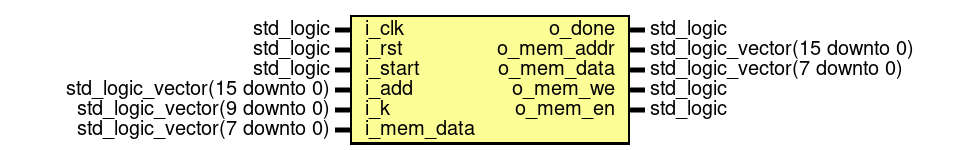
\includegraphics[scale=.45]{resources/entity.png}
    \caption{Diagramma del componente}
    \label{fig:entity}
\end{figure}

\begin{table}[h]
    \centering
    \resizebox{\textwidth}{!}{
        \begin{tabular}{lrl}
            \toprule
            \textbf{Nome Porta} & \textbf{Tipo} & \textbf{Descrizione} \\
            \toprule
            \multicolumn{3}{l}{\textbf{Ingressi Principali}} \\
            \midrule
            \m{i\_start} & 1 bit & Segnale di inizio elaborazione \\
            \addlinespace
            \m{i\_add} & 16 bit & Indirizzo della memoria da cui inizia la porzione da processare \\
            \addlinespace
            \m{i\_k} & 10 bit & Numero di parole da elaborare \\
            \toprule
            \multicolumn{3}{l}{\textbf{Ingressi Ausiliari}} \\
            \midrule
            \m{i\_clk} & 1 bit & Segnale di clock unico per tutto il sistema \\
            \addlinespace
            \m{i\_rst} & 1 bit & Segnale di reset asincrono \\
            \toprule
            \multicolumn{3}{l}{\textbf{Uscita Principale}} \\
            \midrule
            \m{o\_done} & 1 bit & Segnale di terminata elaborazione \\
            \toprule
            \multicolumn{3}{l}{\textbf{Connessioni con la Memoria}} \\
            \midrule
            \m{i\_mem\_data} & 8 bit & Contenuto in ingresso dalla memoria quando letta \\
            \addlinespace
            \m{o\_mem\_en} & 1 bit & Segnale di \textit{enable}, deve essere 1 per comunicare con la memoria \\
            \addlinespace
            \m{o\_mem\_we} & 1 bit & Segnale di \textit{write enable}, deve essere 1 per scrivere, 0 per leggere \\
            \addlinespace
            \m{o\_mem\_addr} & 16 bit & Indirizzo della memoria da cui leggere o in cui scrivere \\
            \addlinespace
            \m{o\_mem\_data} & 8 bit & Dato che verrà scritto in memoria \\
            \bottomrule
        \end{tabular}
    }
    \caption{Descrizione delle porte di interfaccia}
    \label{tab:ports}
\end{table}
\newpage

\subsection{Processi}
Il modulo è composto da un unico processo \textit{design}, con elementi della lista di sensibilità i segnali \m{i\_clk} ed \m{i\_rst}.

La \textit{FSM} (macchina a stati) è sincronizzata in modo da computare uno stato ad ogni ciclo di clock, mentre, essendo il reset asincrono, è presente nella lista di sensibilità in modo da far terminare l'elaborazione nel momento in cui si verifica un fronte di salita del segnale stesso.

Abbiamo scelto di implementare l'intero componente attraverso un unico processo invece di dividerlo in tre sottoprocessi - cambio di stato, \textit{lambda} (funzione di stato prossimo), \textit{delta} (funzione di uscita) - in quanto la bassa complessità dell'elaborazione rispetto ai tempi disponibili permettevano la costruzione di codice più semplice e leggibile, evitando problemi di sincronizzazione o creazione di latch non desiderati.

\subsection{Segnali}
Nella \autoref{tab:signals} vengono presentati i segnali utilizzati all'interno del modulo. 
\begin{table}[h]
    \centering
    \resizebox{\textwidth}{!}{
        \begin{tabular}{lrl}
            \toprule
            \textbf{Nome Segnale} & \textbf{Tipo} & \textbf{Descrizione} \\
            \midrule
            \m{k} & 10 bit & Numero di parole rimanenti da elaborare \\
            \addlinespace
            \m{addr} & 16 bit & Indirizzo da cui leggere o in cui scrivere il prossimo dato \\
            \addlinespace
            \m{data} & 8 bit & Contenuto dell'ultimo valore di parola \m{W} valido \\
            \addlinespace
            \m{cred} & 8 bit & Credibilità \m{C} da assegnare  alla parola corrente \\
            \addlinespace
            \m{current\_state} & \m{state\_type} & Stato corrente dell'elaborazione \\
            \bottomrule
        \end{tabular}
    }
    \caption{Segnali interni}
    \label{tab:signals}
\end{table}

\subsection{Macchina a stati}
Il funzionamento del componente è sintetizzato nella macchina a stati rappresentata in \autoref{fig:fsm}. La descrizione di ogni stato è approfondito nella \autoref{tab:fsm}.
\begin{figure}[H]
    \centering
    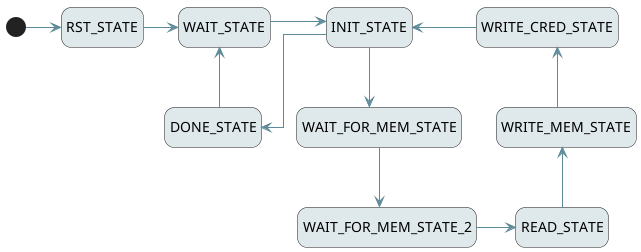
\includegraphics[scale=.65]{resources/fsm.png}
    \caption{Macchina a stati}
    \label{fig:fsm}
\end{figure}
\begin{longtable}{l p{0.75\textwidth}}
        \toprule
        \textbf{Stato} & \textbf{Descrizione} \\
        \midrule
        \m{RST\_STATE} & Stato di reset, accedibile da ogni stato quando \m{i\_rst} $= 1$; quando \m{i\_rst}$=0$ si passa a \m{WAIT\_STATE} \\
        \addlinespace
        \m{WAIT\_STATE} & Stato di attesa di una nuova elaborazione; quando \m{i\_start} $= 1$ vengono inizializzati i segnali \m{k} e \m{addr} con i rispettivi segnali in ingresso, mentre a \m{cred} viene assegnato il valore $31$, infine si passa a \m{INIT\_STATE}\\
        \addlinespace
        \m{INIT\_STATE} & Stato di inizio elaborazione; se \m{k} $\neq 0$ viene attivato il collegamento con la memoria imponendo \m{o\_mem\_en} $=1$ e si passa a \m{WAIT\_FOR\_MEM\_STATE}, altrimenti si impone \m{o\_done} $=1$ e si passa a \m{DONE\_STATE}\\
        \addlinespace
        \m{WAIT\_FOR\_MEM\_STATE} & Stato di attesa di attivazione della memoria, si passa a \m{WAIT\_FOR\_MEM\_STATE\_2}\\
        \addlinespace
        \m{WAIT\_FOR\_MEM\_STATE\_2} & Stato di attesa di ricezione del contenuto della memoria, necessario a causa del ritardo di $2\ ns$ introdotto dalla memoria tra la ricezione della richiesta di dati e l'invio degli stessi; si passa a \m{READ\_STATE}\\
        \addlinespace
        \m{READ\_STATE} & Stato di lettura del contenuto della memoria e decisione dei valori in uscita verso la memoria; se è un valore non valido si mantiene in \m{data} l'ultimo valore valido e si decrementa \m{cred}, altrimenti si impone il valore corrente a \m{data} e si resetta \m{cred}$= 31$. Viene attivata la scrittura in memoria imponendo \m{o\_mem\_we} $= 1$ e si passa a \m{WRITE\_MEM\_STATE}\\
        \addlinespace
        \m{WRITE\_MEM\_STATE} & Stato di scrittura del dato in memoria, in cui viene scritto il valore presente nel segnale \m{data}, viene aggiornato il segnale \m{addr} ad \m{addr} $+ 1$ e si passa a \m{WRITE\_CRED\_STATE}\\
        \addlinespace
        \m{WRITE\_CRED\_STATE} & Stato di scrittura della credibilità in memoria, in cui viene scritto il valore presente nel segnale \m{cred},viene aggiornato il segnale \m{addr} ad \m{addr} $+ 1$ e si passa a \m{INIT\_STATE}\\
        \addlinespace
        \m{DONE\_STATE} & Stato di terminazione dell'elaborazione, quando \m{i\_start} viene posto a zero si passa in \m{WAIT\_STATE} ed il componente è pronto ad una nuova elaborazione \\
        \bottomrule
    \caption{Stati della \textit{FSM}}
    \label{tab:fsm}
\end{longtable}

In ogni stato vengono imposti i valori desiderati ai segnali che saranno utilizzati nello stato successivo: infatti tutti i segnali vengono aggiornati sul fronte di salita del clock, il quale coincide con il cambio di stato. Ad esempio per far sì che durante lo stato di \m{WRITE\_MEM\_STATE} venga scritto il dato in memoria è necessario imporre \m{o\_mem\_we} $= 1$ nello stato di \m{READ\_STATE}, in modo che al successivo fronte di salita del clock (quindi al conseguente passaggio di stato) il segnale venga imposto ad uno.

\section{Risultati sperimentali}

\subsection{Report di sintesi}
Dopo aver sintetizzato il design del progetto, il circuito è stato simulato utilizzando il test bench fornito. Il circuito si comporta correttamente, superando il test sia con la simulazione comportamentale (\textit{behavioral simulation}) che con la simulazione post-sintesi (\textit{post-synthesis simulation}). Di seguito, sono riportate le tabelle con il timing report e l'utilizzo delle risorse. Nella \autoref{tab:timing_report} è mostrato il timing report del design; analizzandolo, si può notare che il Worst Negative Slack (\textit{WNS}) è di 15,413 ns. Un WNS di 15,413 ns con un periodo di clock di 20 ns indica che il circuito impiega (20 ns - 15,413 ns = 4,587 ns) per completare l'esecuzione di uno stato della FSM del design, dato che la FSM è stata sincronizzata in modo da eseguire uno stato per ogni ciclo di clock, come è possibile notare dalla \autoref{fig:state_clk_sync}.

\vspace{1em}

\begin{table}[ht]
    \centering
    \resizebox{\textwidth}{!}{
        \begin{tabular}{lll}
            \toprule
            \textbf{Setup}                        & \textbf{Hold}                    & \textbf{Pulse Width}                              \\
            \midrule
            Worst Negative Slack (WNS): 15,413 ns & Worst Hold Slack (WHS): 0,148 ns & Worst Pulse Width Slack (WPWS): 9,500 ns          \\
            \addlinespace
            Total Negative Slack (TNS): 0,000 ns  & Total Hold Slack (THS): 0,000 ns & Total Pulse Width Negative Slack (TPWS): 0,000 ns \\
            \addlinespace
            Number of Failing Endpoints: 0        & Number of Failing Endpoints: 0   & Number of Failing Endpoints: 0                    \\
            \addlinespace
            Total Number of Endpoints: 119        & Total Number of Endpoints: 119   & Total Number of Endpoints: 79                     \\
            \bottomrule
        \end{tabular}
    }
    \caption{Design Timing Summary}
    \label{tab:timing_report}
\end{table}
\begin{figure}[ht]
    \centering
    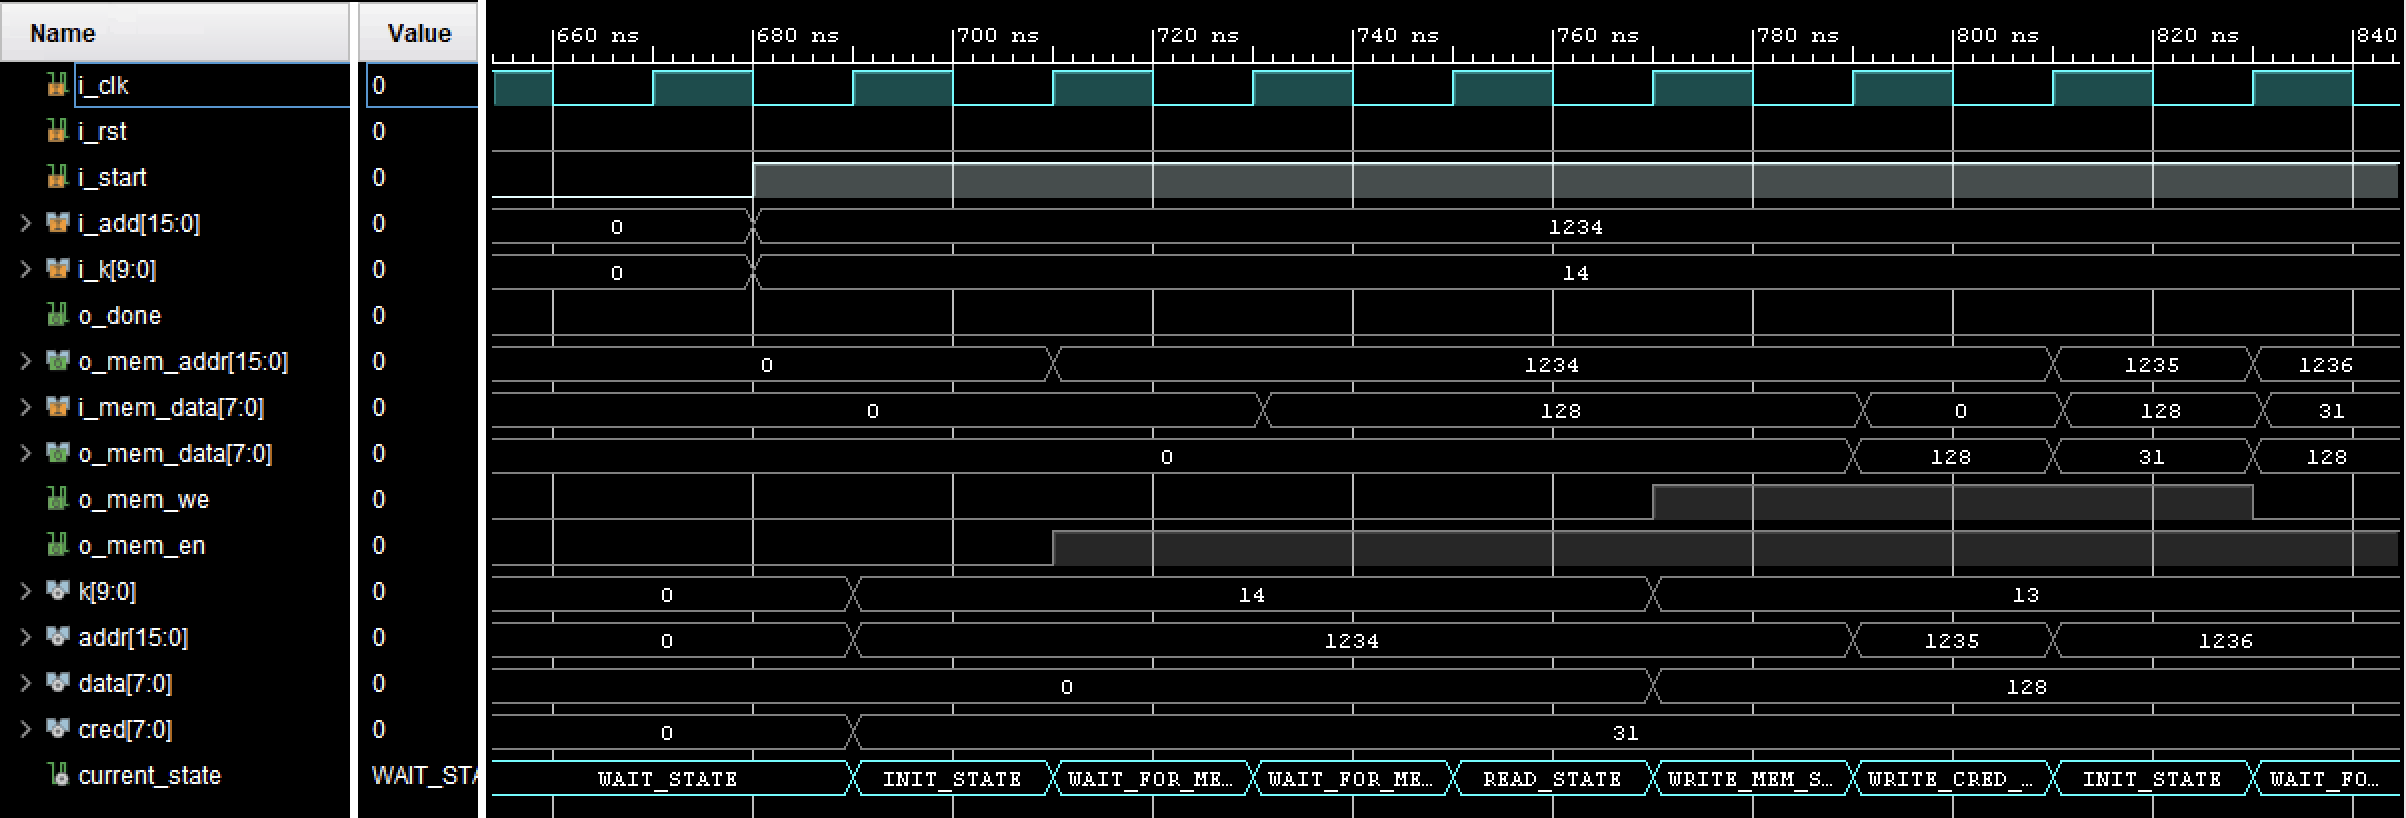
\includegraphics[width=\textwidth]{resources/state_clk_sync.png}
    \caption{Sincronizzazione della FSM con il clock}
    \label{fig:state_clk_sync}
\end{figure}
\vspace{1em}
Da questo valore è anche possibile calcolare il periodo di clock minimo che il design può supportare. Sapendo che la memoria (RAM) ha un ritardo massimo di 2 ns nelle operazioni di scrittura e lettura, il periodo di clock minimo è dato da:

\begin{equation}
    T_{clk} = 20\ ns + 2\ ns - 15,413\ ns = 6,587\ ns
\end{equation}

e la frequenza di clock massima supportata dal design è:

\begin{equation}
    f_{clk} = \frac{1}{T_{clk}} = \frac{1}{6,587\ ns} \approx 151,8\ MHz
\end{equation}

\vspace{1em}
Dalla \autoref{tab:utilization_report} si può invece osservare come il design utilizzi 78 registri di tipo \textit{Flip-Flop} e 86 \textit{LUTs}, il che significa che il design non presenta alcun tipo di \textit{Latch}. Questo evita comportamenti imprevedibili e indesiderati, assicurando inoltre che il design sia completamente sincrono. Per evitare la creazione di Latch e sincronizzare correttamente il design con il periodo di clock, è stato necessario implementare la FSM in un singolo processo invece di dividerla in più processi.

\begin{table}[ht]
    \centering
    \begin{tabular}{lrrrr}
        \toprule
        \textbf{Site Type}          & \textbf{Used} & \textbf{Fixed} & \textbf{Available} & \textbf{Util\%} \\
        \midrule
        Slice LUTs*                 & 86            & 0              & 134600             & 0,06            \\
        \addlinespace
        \quad LUT as Logic          & 86            & 0              & 134600             & 0,06            \\
        \addlinespace
        \quad LUT as Memory         & 0             & 0              & 46200              & 0,00            \\
        \midrule
        Slice Registers             & 78            & 0              & 269200             & 0,03            \\
        \addlinespace
        \quad Register as Flip Flop & 78            & 0              & 269200             & 0,03            \\
        \addlinespace
        \quad Register as Latch     & 0             & 0              & 269200             & 0,00            \\
        \midrule
        F7 Muxes                    & 0             & 0              & 67300              & 0,00            \\
        \addlinespace
        F8 Muxes                    & 0             & 0              & 33650              & 0,00            \\
        \bottomrule
    \end{tabular}
    \caption{Resource Utilization Summary}
    \label{tab:utilization_report}
\end{table}

\subsection{Simulazioni}
Per assicurarsi che il design fosse corretto e privo di errori, sono stati simulati vari test bench con l'obiettivo di verificare diversi corner cases. Inoltre, è stato sviluppato un codice in Python per generare automaticamente una serie di test bench, inizializzando la RAM con messaggi composti da \m{K} $\in [1, 100]$ parole e assegnando a ciascuna parola un valore \m{W} $\in [0, 255]$, come da specifica. I test bench generati da Python sono stati successivamente simulati con GHDL, uno strumento utilizzato per la simulazione e verifica dei design VHDL.

\subsubsection{Tesh bench fornito}
In questo test bench viene illustrato il funzionamento del design con una sequenza definita come \textit{"normale"}, in cui viene mostrato il corretto utilizzo di tutti i segnali per interfacciarsi con la RAM. Nella \autoref{fig:start_signal} e nella \autoref{fig:end_signal} è possibile osservare i segnali di inizio e fine elaborazione, che vengono attivati correttamente durante l'esecuzione del design. In particolare, il segnale di inizio elaborazione (\m{i\_start}), attivato una volta che il segnale di reset (\m{i\_rst}) è disattivato, avvia correttamente l'elaborazione del design, come si può notare dal cambiamento degli stati; in dettaglio, la FSM passa da \m{WAIT\_STATE} a \m{INIT\_STATE}, procedendo con la lettura della RAM. Una volta che il design ha terminato l'elaborazione della sequenza, il segnale di terminazione dell'elaborazione (\m{o\_done}) viene attivato e, infine, il segnale \m{i\_start} viene disattivato, rendendo il design pronto per una nuova elaborazione.

\vspace{0.5em}

\begin{figure}[htbp]
    \centering
    \begin{minipage}{0.5\textwidth}
        \centering
        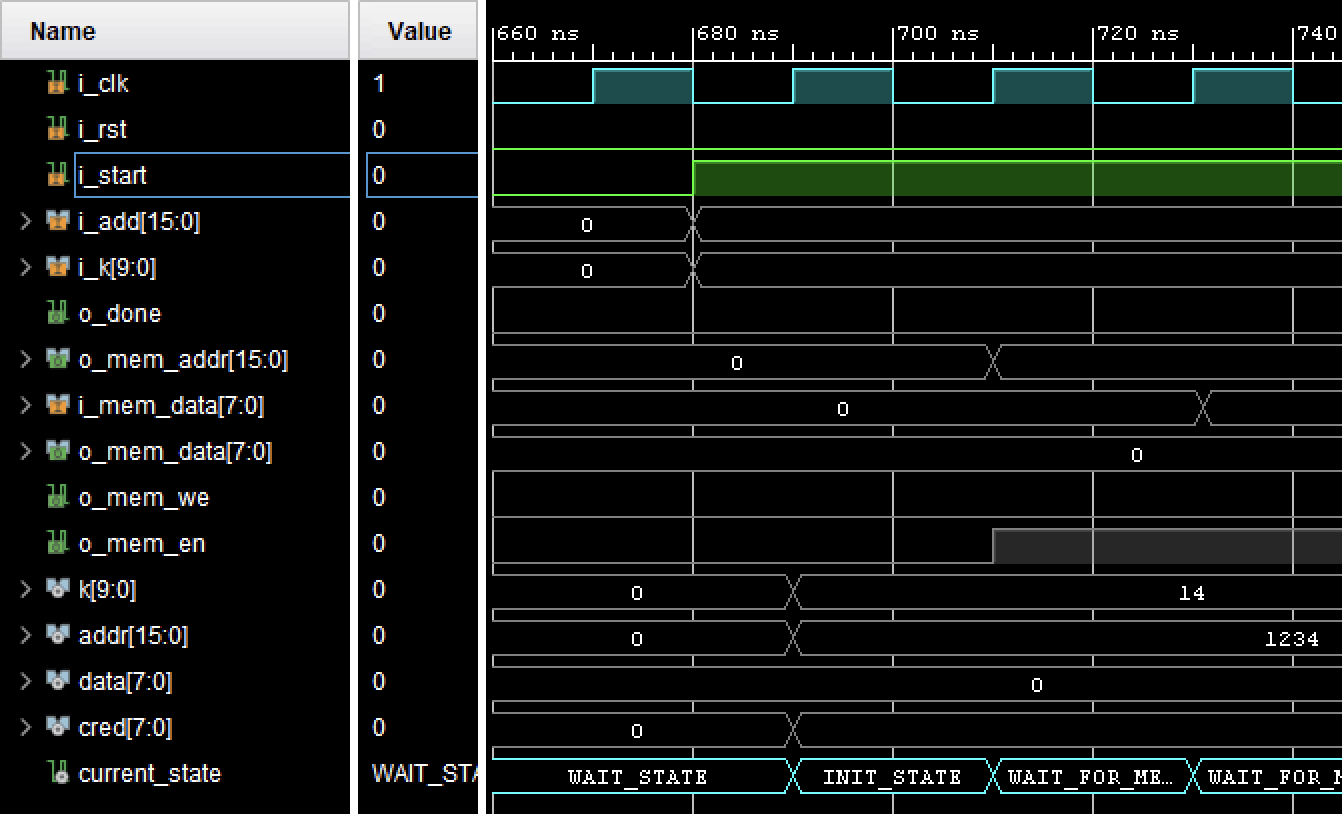
\includegraphics[height=4.7cm]{resources/start_signal.png}
        \caption{Segnali di inizio elaborazione}
        \label{fig:start_signal}
    \end{minipage}\hfill
    \begin{minipage}{0.5\textwidth}
        \centering
        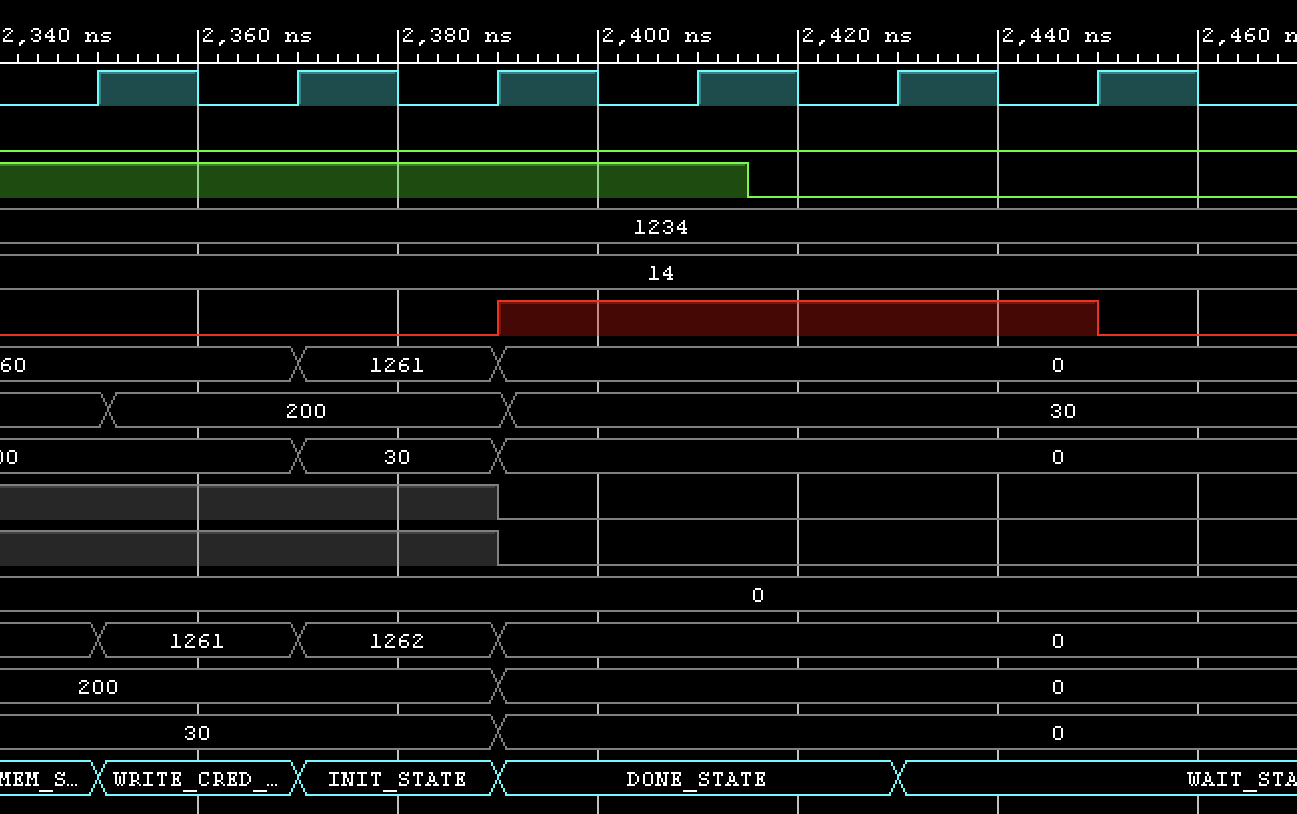
\includegraphics[height=4.7cm]{resources/end_signal.png}
        \caption{Segnali di fine elaborazione}
        \label{fig:end_signal}
    \end{minipage}
    \label{fig:normal_sequence}
\end{figure}

\subsubsection{Sequenza di lunghezza nulla}
In questo test bench viene illustrato il comportamento del design quando la sequenza è vuota, ovvero quando il segnale che indica la lunghezza della sequenza (\m{i\_k}) è pari a 0. Come mostrato nella \autoref{fig:empty_sequence}, il design avvia correttamente l'elaborazione non appena il segnale di reset viene disattivato e quello di start attivato. Tuttavia, appena rileva che \m{k} = 0 leggendo dalla RAM, il design conclude immediatamente l'elaborazione, attivando il segnale \m{o\_done}, che viene poi disattivato quando \m{i\_start} è disattivato. La FSM, una volta attivato \m{i\_start}, passa da \m{WAIT\_STATE} a \m{INIT\_STATE}; da quest'ultimo stato, procede a \m{DONE\_STATE} se \m{k} = 0, altrimenti passa a \m{WAIT\_FOR\_MEM\_STATE}, come si può osservare nella figura.

\vspace{0.5em}
\begin{figure}[htbp]
    \centering
    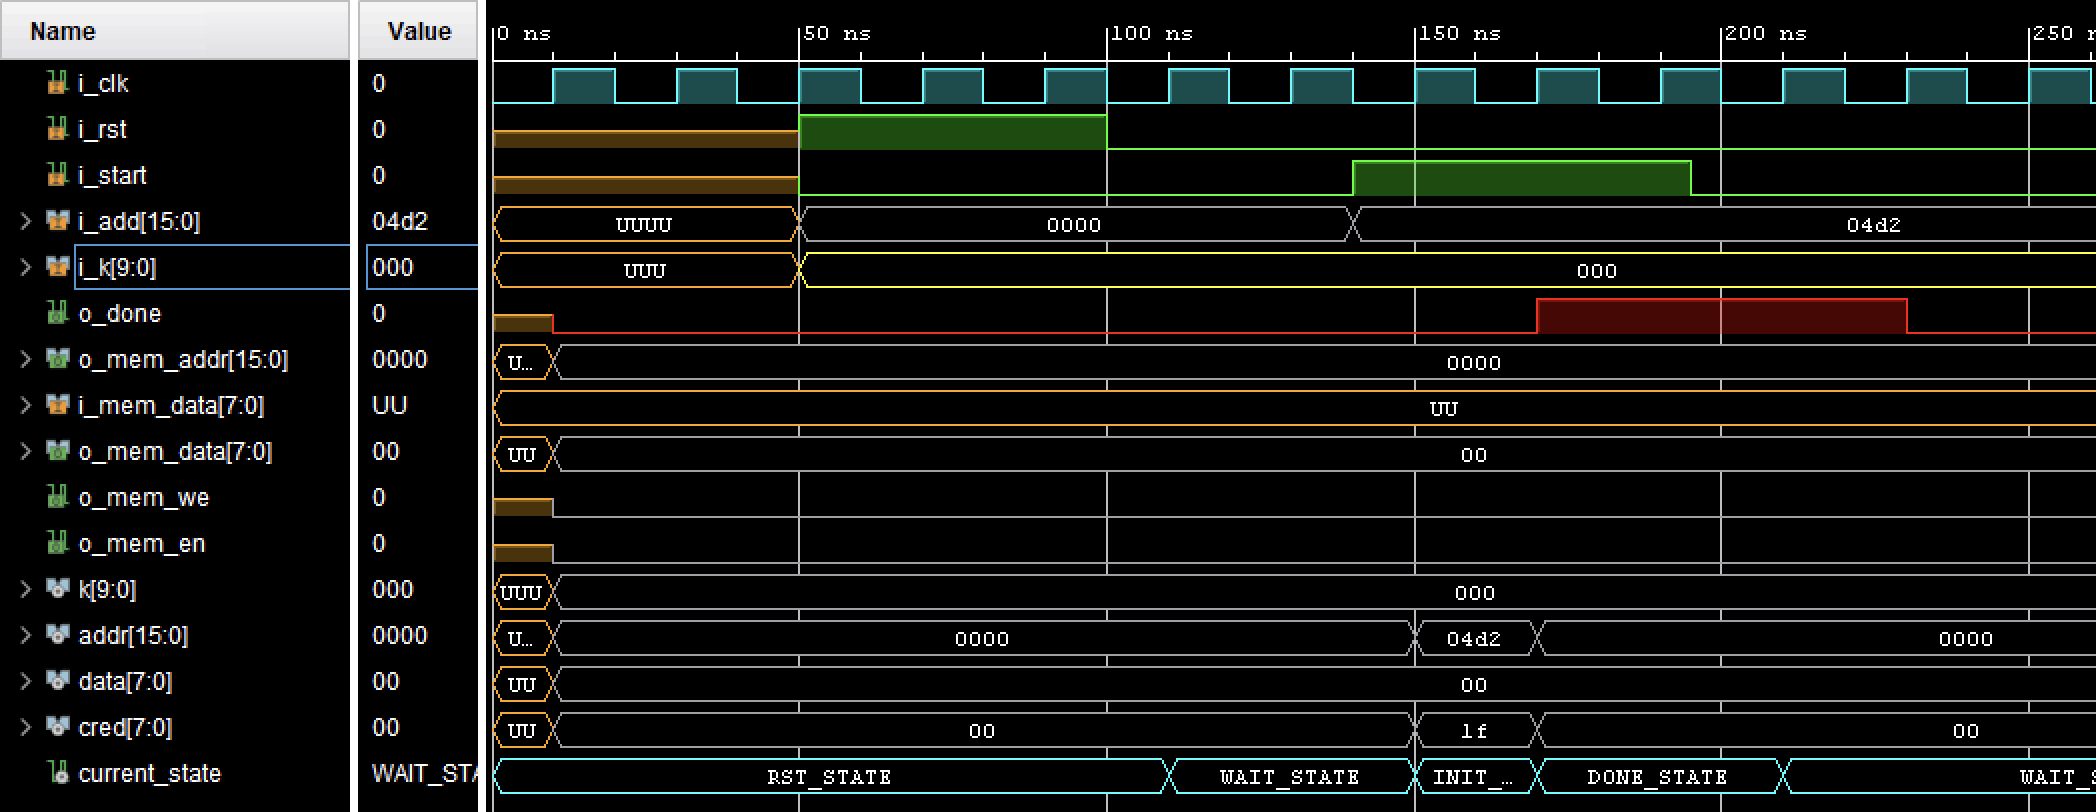
\includegraphics[width=\textwidth]{resources/empty_sequence.png}
    \caption{Sequenza di lunghezza nulla}
    \label{fig:empty_sequence}
\end{figure}

\subsubsection{Credibilità che raggiunge 0}
Questo test bench illustra il comportamento del design quando la credibilità viene decrementata ogni volta che si incontra uno zero in \m{W}, finché non si rileva un valore diverso da 0, momento in cui la credibilità viene reinizializzata a 31 per poi essere nuovamente decrementata se si incontra un altro zero. Secondo la specifica, una volta che la credibilità raggiunge 0, il design deve mantenere tale valore fino a che non si rileva un valore in \m{W} diverso da 0 o fino al termine della sequenza. Come previsto, alla fine della sequenza, il design deve attivare il segnale di fine elaborazione. Nella \autoref{fig:cred_0_start} e nella \autoref{fig:cred_0_end} è possibile osservare come il design si comporti correttamente, continuando a decrementare la credibilità fino a 0 e mantenendola a 0, dato che non si verificano valori diversi da 0 in \m{W}.

\vspace{0.5em}
\begin{figure}[htbp]
    \centering
    \begin{minipage}{0.6\textwidth}
        \centering
        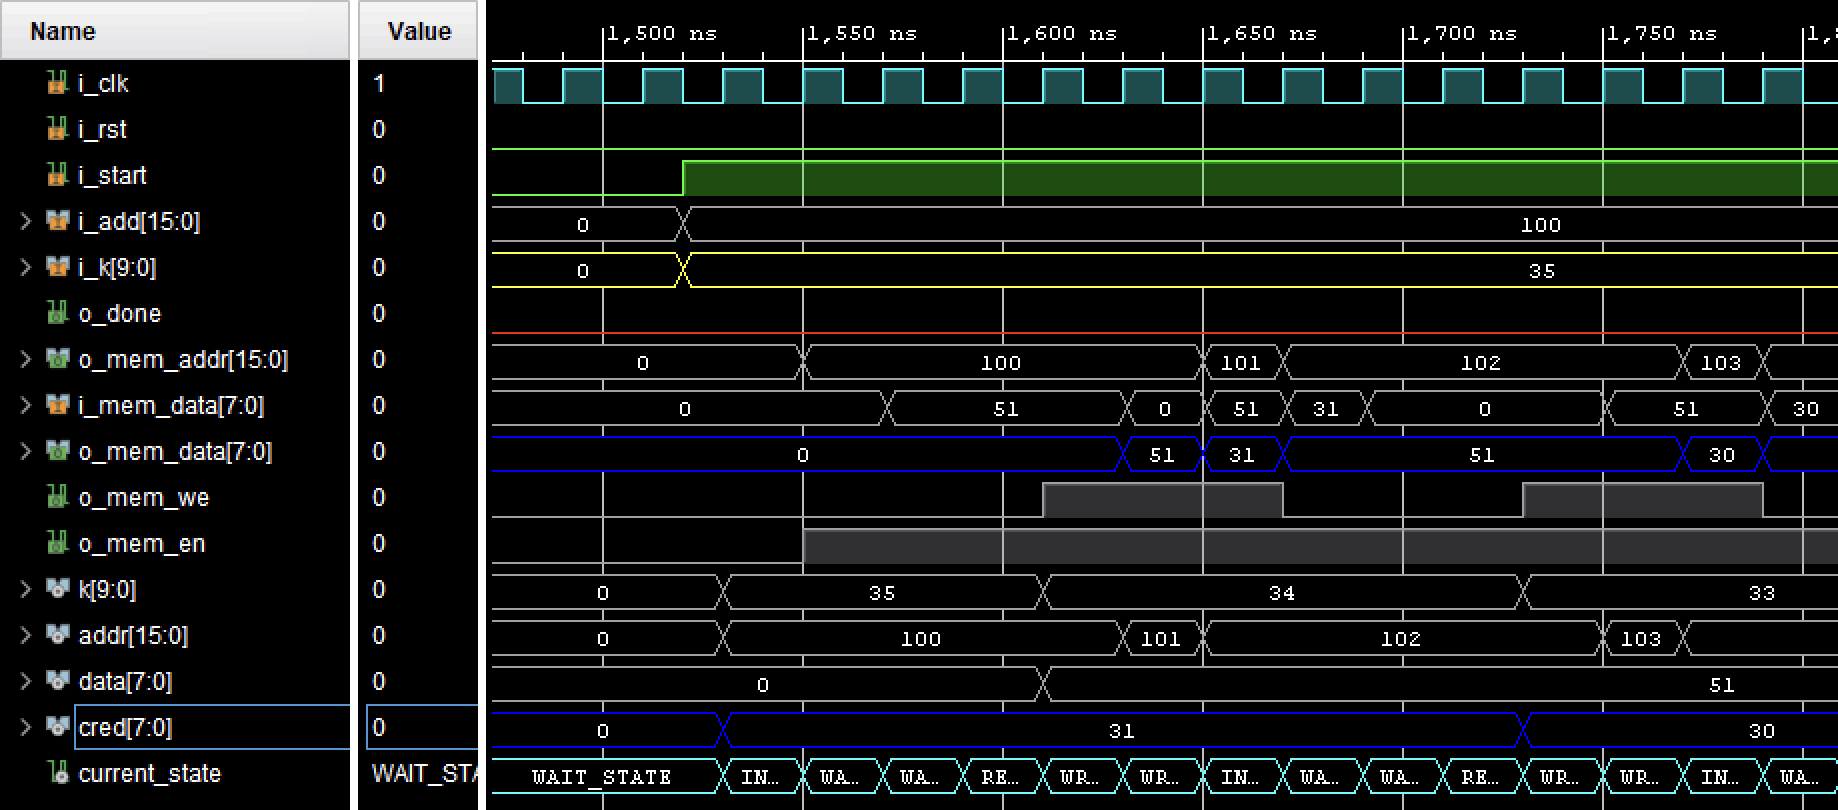
\includegraphics[height=4.5cm]{resources/cred_0_start.png}
        \caption{Segnali di inizio elaborazione}
        \label{fig:cred_0_start}
    \end{minipage}\hfill
    \begin{minipage}{0.4\textwidth}
        \centering
        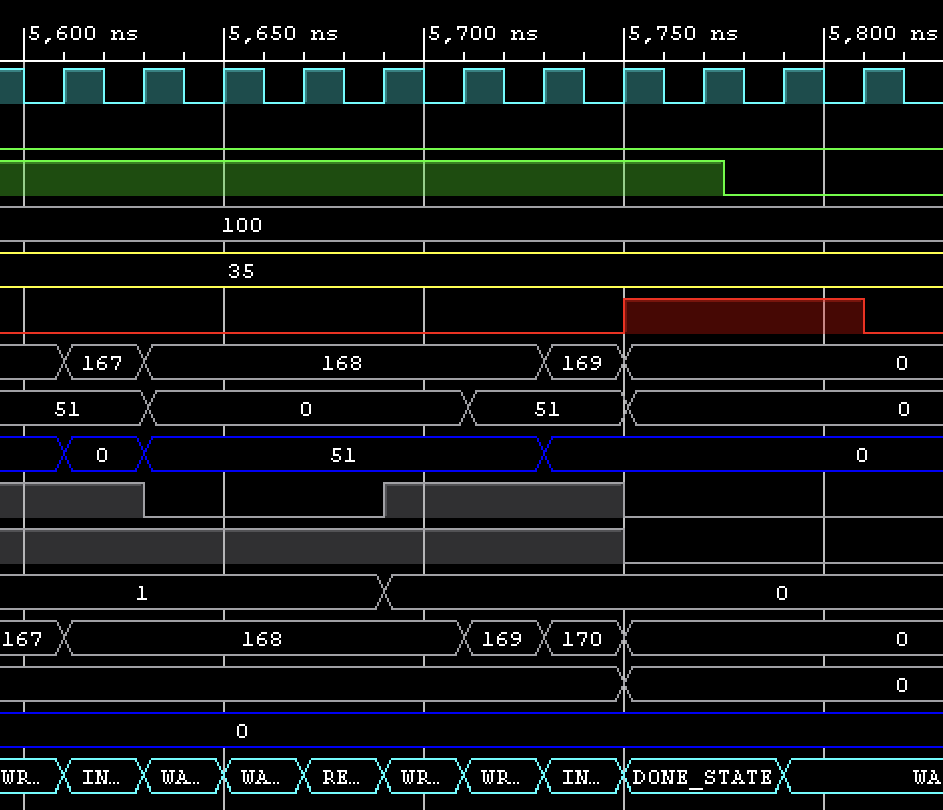
\includegraphics[height=4.5cm]{resources/cred_0_end.png}
        \caption{Segnali di fine elaborazione}
        \label{fig:cred_0_end}
    \end{minipage}
    \label{fig:cred_0_sequence}
\end{figure}

\subsubsection{Test bench con sequenza nulla iniziale}
In questo test bench si è voluto verificare il funzionamento del design quando la sequenza di parole \m{W} inizia con un valore pari a 0. In questo scenario, il design deve avviare l'elaborazione della sequenza mantenendo il valore \m{W} nullo e impostando e mantenendo la credibilità a 0, fino a quando non si legge dalla RAM un valore di \m{W} diverso da 0. A quel punto, il design si comporta come mostrato nei test bench precedenti. Nella \autoref{fig:value_0_start} e nella \autoref{fig:value_0_mid} si verifica che il design opera in modo appropriato: in particolare, si può notare come sia la credibilità che il valore di \m{W} rimangano a 0. Questo è evidenziato anche dal segnale \m{o\_mem\_data} (segnale che indica il valore da scrivere nella RAM all'indirizzo \m{o\_mem\_addr}), che resta a 0 fino a quando non viene letto dalla RAM un valore diverso da 0; nel caso del test bench, questo valore è 2 e la credibilità viene poi posta a 31.

\vspace{0.5em}
\begin{figure}[htbp]
    \centering
    \begin{minipage}{0.5\textwidth}
        \centering
        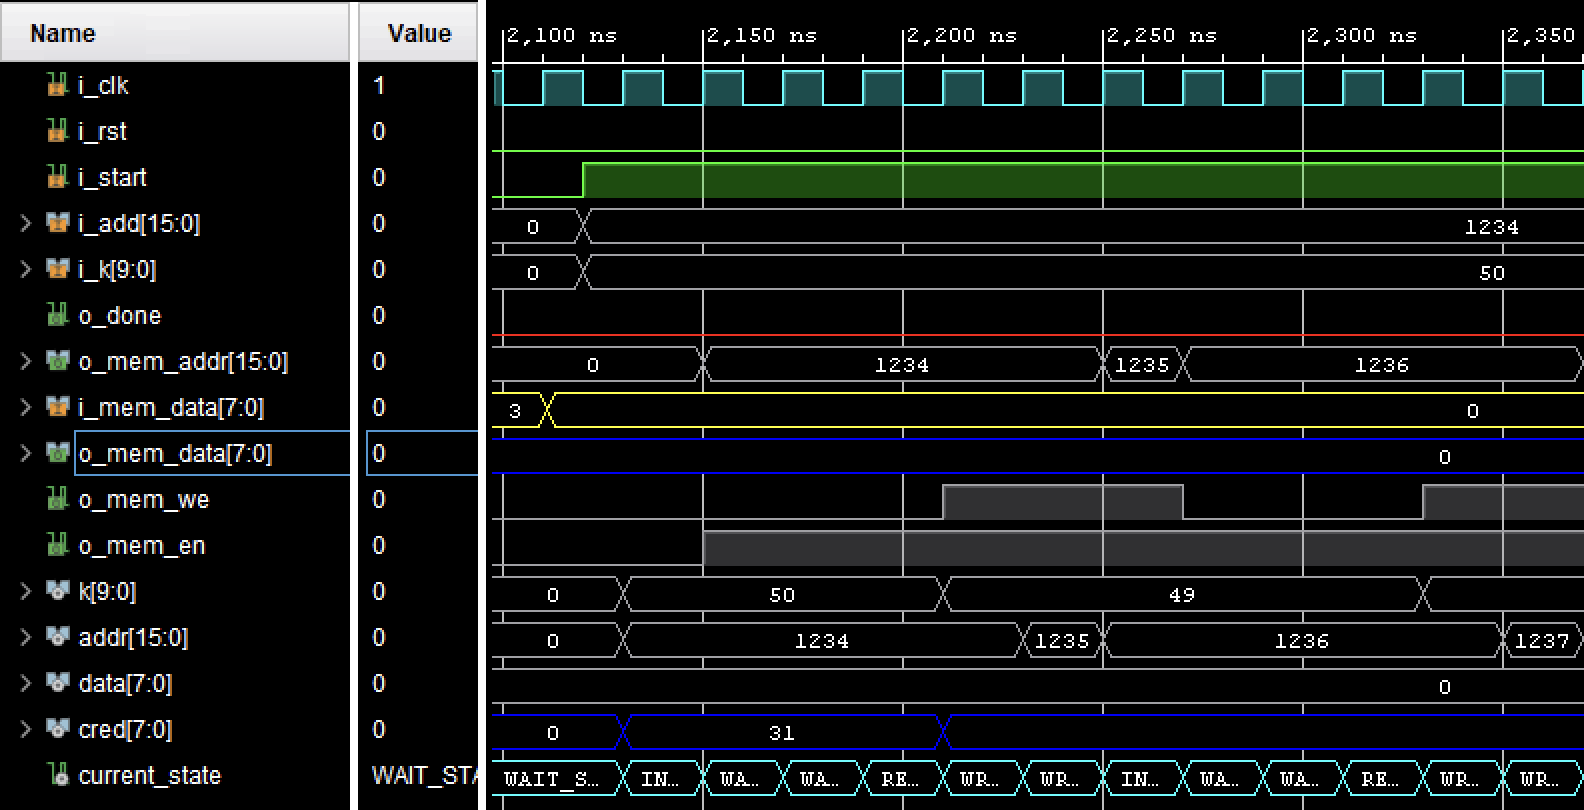
\includegraphics[height=4.3cm]{resources/value_0_start.png}
        \caption{Segnali di inizio elaborazione}
        \label{fig:value_0_start}
    \end{minipage}\hfill
    \begin{minipage}{0.5\textwidth}
        \centering
        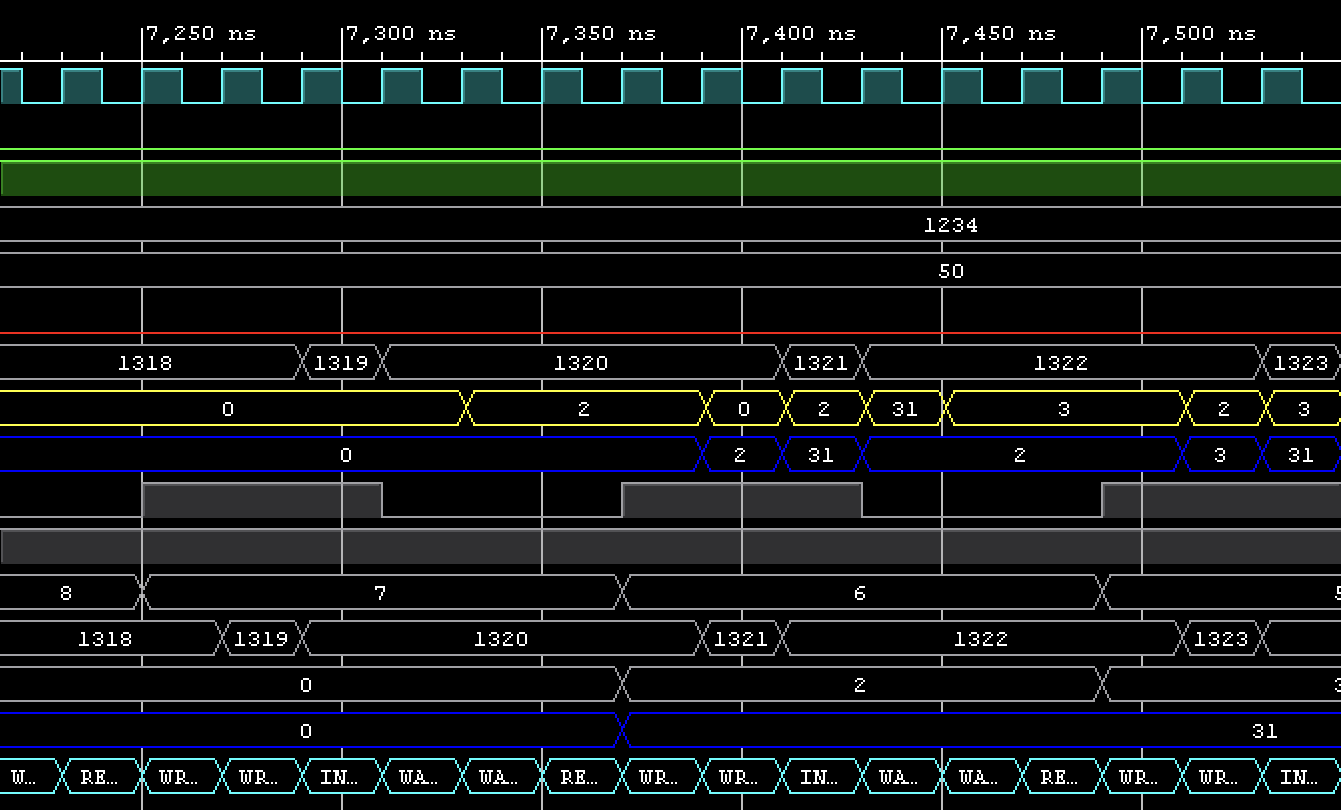
\includegraphics[height=4.3cm]{resources/value_0_mid.png}
        \caption{Fine elaborazione di una sequenza di 0}
        \label{fig:value_0_mid}
    \end{minipage}
    \label{fig:value_0_sequence}
\end{figure}

\subsubsection{Sequenze multiple}
In questo test bench si verifica come il design si comporta nell'elaborazione di sequenze multiple. Dalla specifica, il design, una volta completata l'elaborazione della prima sequenza, deve attivare il segnale di fine elaborazione (\m{o\_done}). Quando \m{o\_done} viene attivato, il segnale \m{i\_start} viene disattivato, seguito dalla disattivazione del segnale di fine elaborazione, il che indica che il modulo è pronto per una nuova elaborazione. Quando \m{i\_start} viene attivato una seconda volta, il modulo avvia la seconda elaborazione. Secondo la specifica, la seconda elaborazione non deve attendere il reset del modulo; questo è verificabile osservando come il modulo, una volta terminata l'elaborazione, passi da \m{DONE\_STATE} a \m{WAIT\_STATE}, e successivamente, con la riattivazione di \m{i\_start}, la FSM passi da \m{WAIT\_STATE} a \m{INIT\_STATE}, procedendo con l'elaborazione della nuova sequenza.

\vspace{0.5em}
\begin{figure}[htbp]
    \centering
    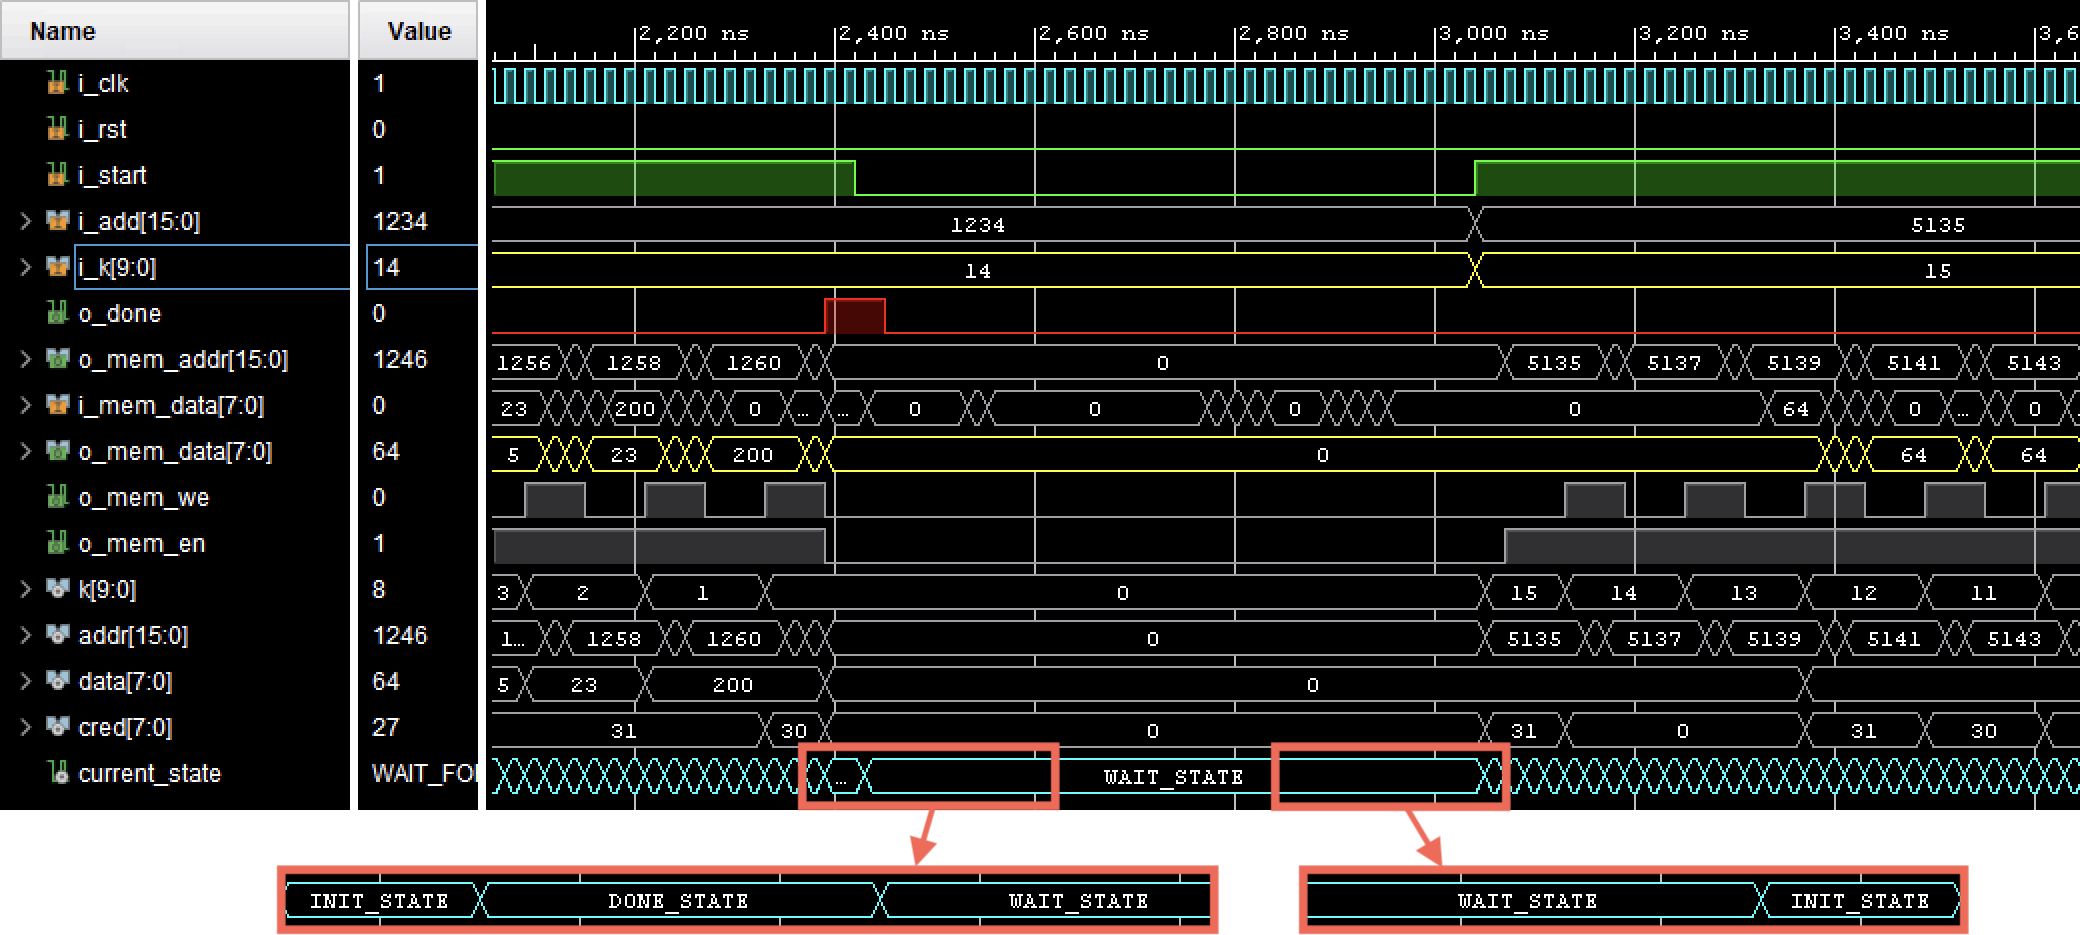
\includegraphics[width=\textwidth]{resources/multiple_sequence.png}
    \caption{Sequenze multiple}
    \label{fig:multiple_sequences}
\end{figure}

\subsubsection{Segnale di reset}
In questo test bench si verifica il corretto funzionamento del design in presenza del segnale di reset asincrono. Come si può notare dalla \autoref{fig:reset}, nel test bench viene attivato il segnale di reset \m{i\_rst} anche se non sincronizzato con il periodo di clock. A seguito dell'attivazione del reset, il modulo viene re-inizializzato, disattivando correttamente tutti i segnali necessari. Tra questi segnali, vi sono quelli che si interfacciano con la RAM, come \m{o\_mem\_data}, \m{o\_mem\_we} e \m{o\_mem\_en}, oltre ai segnali interni al modulo, come \m{k}, \m{addr}, \m{data} e \m{cred}. Il corretto funzionamento del design è evidente anche dagli stati della FSM implementata nel modulo. La FSM passa dallo stato \m{WRITE\_CRED\_STATE} a \m{RST\_STATE} non appena il segnale di reset viene portato a 1. Successivamente, appena il segnale di reset viene disattivato e il clock è attivo, la FSM passa da \m{RST\_STATE} a \m{WAIT\_STATE}, indicando che il modulo è pronto per una nuova elaborazione.

\vspace{0.5em}

\begin{figure}[htbp]
    \centering
    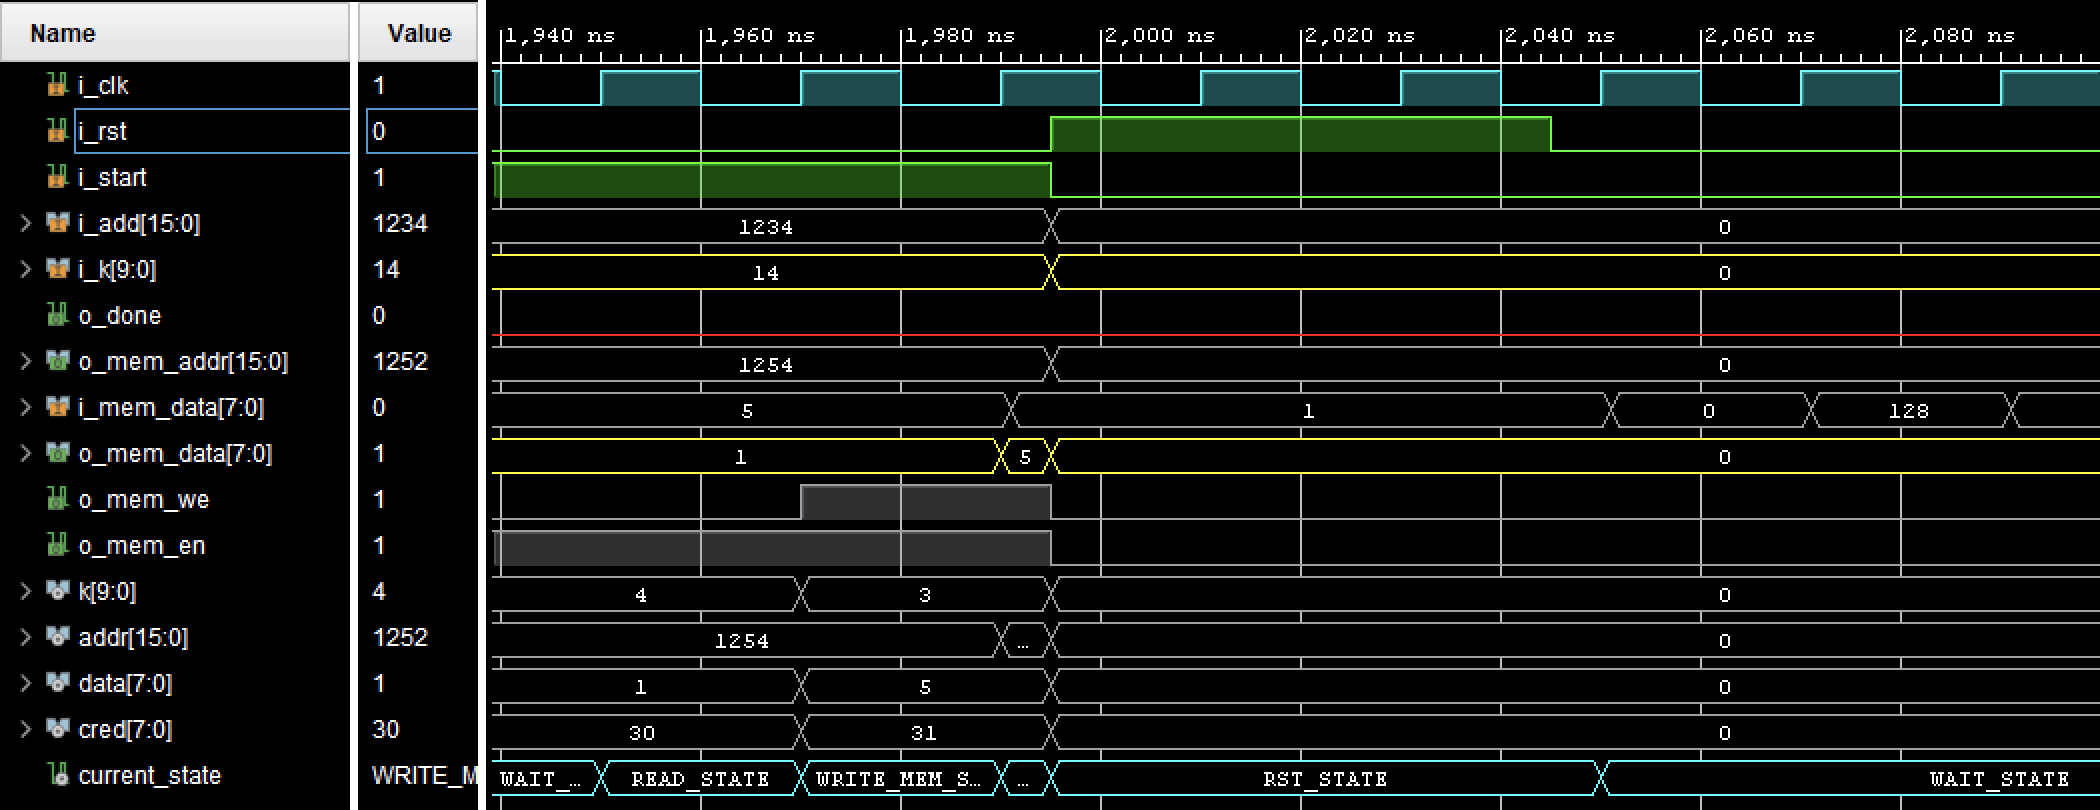
\includegraphics[width=\textwidth]{resources/reset.png}
    \caption{Segnale di reset}
    \label{fig:reset}
\end{figure}

\subsubsection{Segnale di start nello stato di reset}
In questo test bench si verifica il corner case in cui il segnale di inizio elaborazione rimane attivo per tutta la durata dell'attivazione del segnale di reset. Secondo la specifica, il sistema funziona correttamente quando, dopo che il segnale di reset viene disattivato, il modulo avvia l'elaborazione al momento in cui il segnale di start viene portato a 1. Tuttavia, non è specificato il comportamento nel caso in cui il segnale di start non venga mai abbassato, anche dopo l'attivazione del reset. Abbiamo quindi gestito questo scenario con la continuazione dell'elaborazione precedente, senza aspettare che il segnale di start venga abbassato e riattivato, come si può osservare nella \autoref{fig:start_in_reset}. Questa scelta è stata fatta immaginando il modulo in un contesto realistico. Ad esempio, se il modulo fosse responsabile di monitorare la corretta lettura di un dispositivo di rilevamento del battito cardiaco (con valori compresi tra 0 e 255) e dovesse segnalare un tecnico quando la credibilità del valore scende a 0, in caso di un reset del modulo senza che la periferica invii un nuovo segnale di start, il sistema continuerebbe a svolgere correttamente il suo compito.

\vspace{0.5em}

\begin{figure}[htbp]
    \centering
    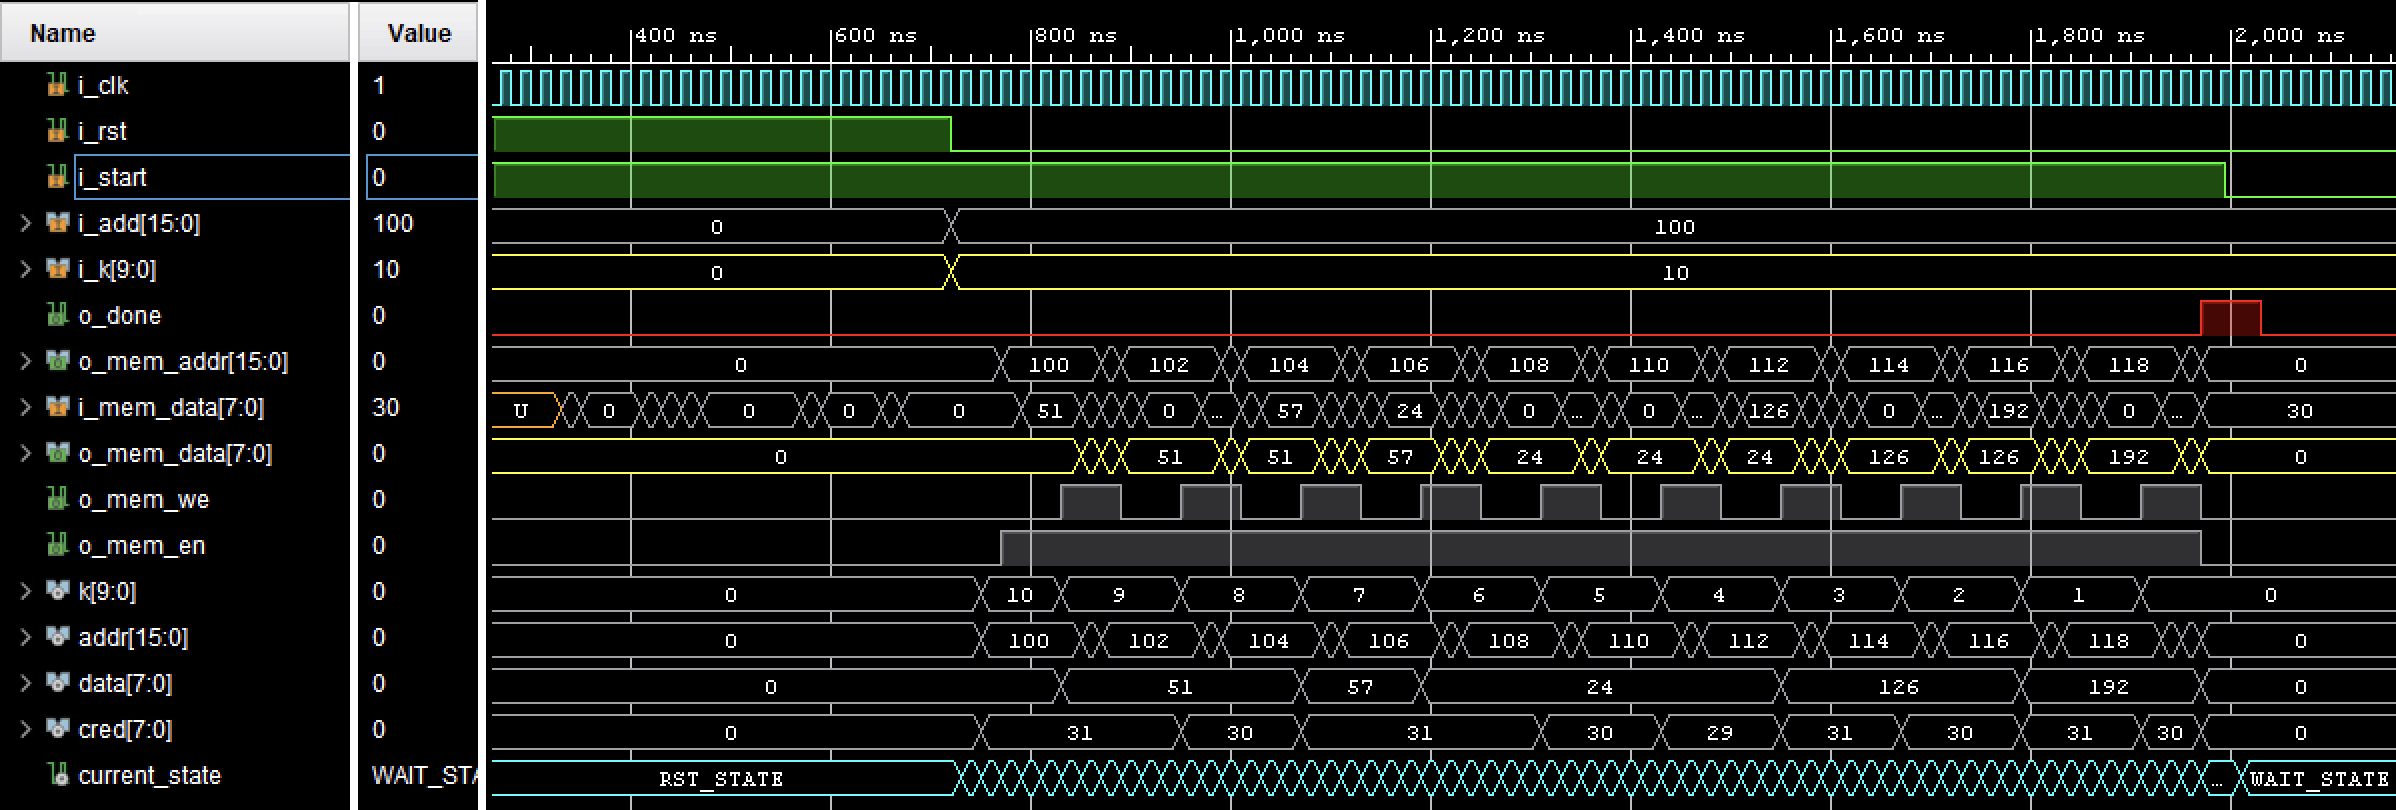
\includegraphics[width=\textwidth]{resources/start_in_reset.png}
    \caption{Segnale di start nello stato di reset}
    \label{fig:start_in_reset}
\end{figure}

\subsubsection{Altri test bench}
Oltre ai test bench mostrati precedentemente, il modulo è stato testato anche con sequenze di lunghezze variabili, da valori bassi fino a lunghezze di circa \m{K} $\approx 1000$. Il modulo è stato inoltre sottoposto a test con più di due sequenze e con segnali di reset casuali durante l'elaborazione.

\section{Conclusioni}
Il design sintetizzato funziona correttamente sia nei test di simulazione comportamentale che in quelli post-sintesi (sia \textit{timing} che \textit{functional}), dimostrando come il design rispetti pienamente le specifiche, compresi i vincoli riguardanti il periodo di clock, che risultano soddisfatti, come analizzato nel paragrafo dedicato al report di sintesi. Per garantire una sincronizzazione corretta ed efficiente, il modulo è stato implementato utilizzando un singolo processo; data la semplicità del progetto, questo approccio si è rivelato sufficiente. Tuttavia, se fossero stati richiesti vincoli sul periodo di clock più restrittivi, sarebbe stato necessario adottare un approccio diverso. Inoltre, si sarebbe potuto analizzare la FSM per identificare eventuali ridondanze, ottimizzando l'uso dei registri e rendendo il modulo più compatto da questo punto di vista.

\end{document}